\documentclass[12pt, a4paper]{article}
\usepackage[utf8]{inputenc}
\usepackage[spanish]{babel}
\usepackage{csquotes}
\usepackage[style=apa,backend=biber]{biblatex}
\addbibresource{./referencie.bib}
\usepackage[T1]{fontenc}
\usepackage{amsmath}
\usepackage{amsfonts}
\usepackage{booktabs}
\usepackage{float}
\usepackage{amssymb}
\usepackage[a4paper, margin=2.54cm]{geometry}
\usepackage{setspace}
\usepackage{titlesec}
\usepackage{graphicx}
\usepackage{pgfplots}
\usepackage{pgf-pie}
\usepackage{booktabs}
\usepackage{enumitem}
\usepackage{pdflscape} % Para landscape
\usepackage{multirow} % Para combinar celdas
\usepackage{array} % Para ajustar anchos de columnas
\usepackage{listings}
\usepackage{xcolor}
\usepackage{pdfpages}
% Configuración de listings
\lstset{
    language=Python,           % Lenguaje de programación
    basicstyle=\ttfamily\small, % Estilo básico
    numbers=left,              % Numeración de líneas
    numberstyle=\tiny\color{gray},  % Estilo de los números
    stepnumber=1,              % Paso para la numeración
    frame=single,              % Marco alrededor del código
    breaklines=true,           % Dividir líneas largas
    captionpos=b,              % Posición de la leyenda
    showstringspaces=false,    % No mostrar espacios en cadenas
    backgroundcolor=\color{lightgray!10}, % Color de fondo
    keywordstyle=\color{blue}, % Estilo de palabras clave
    commentstyle=\color{green!60!black}, % Estilo de comentarios
    stringstyle=\color{red}    % Estilo de cadenas
}
\renewcommand{\arraystretch}{1.5} % Ajusta el espaciado entre filas
% Configuración de APA 7ma edición

\setlength{\parindent}{0.5in}
\titleformat*{\section}{\normalfont\bfseries}
\titleformat*{\subsection}{\normalfont\bfseries}
\titleformat*{\subsubsection}{\normalfont\bfseries}
\pgfplotsset{compat=1.18}

\begin{document}
\onehalfspacing

\begin{titlepage}
    \begin{center}
        \vspace{0.5in}
        \small “Año del Bicentenario, de la consolidación de nuestra Independencia, y de la conmemoración de las heroicas batallas de Junín y Ayacucho”
  
        \Large Universidad Nacional Hermilio Valdizán
        
        \Large Facultad de Economía
        
        
        \begin{figure}[h!]
            \begin{center}
                
\includegraphics[width=0.3\textwidth]{images/unheval.jpg}
            \end{center}
        \end{figure}
        
        \Large{ANÁLISIS CUANTITATIVO DE LA SITUACIÓN DE EMPLEO Y DESEMPLEO DE PROFESIONALES EN EL DISTRITO DE HUÁNUCO}
        \vspace{0.5cm} 

        \large\textbf{Docente:}

        \large\textbf\author{Cueva Laguna, Jeel E. }
        
        \large\textbf{Autores:}

        \large\textbf\author{Ayala Torres Yenifer Y.}

        \large\textbf\author{Carrillo Alejo Joysi M.}

        \large\textbf\author{, Gonzales Jara Jhan C.}
        
        \large\textbf\author{Maíz Villarán, Edith Y.}

        \large\textbf\author{Mallqui Rubin Araceli B.}
        
        \large\textbf\author{Martell Schauss A. Francesca}

        \large\textbf\author{Rojas León Rut E.}

        \large\textbf\author{Rojas Nieto Jhojan P}
        
        \Large Huánuco - Perú 
        
        \large 2024
    \end{center}
\end{titlepage}

\tableofcontents
\newpage

\begin{abstract}
    Este informe muestra el estudio cuantitativo de la situación de empleo y desempleo de profesionales del distrito de Huánuco, en el 2024. El objetivo general de la investigación es conocer la cantidad de profesionales del distrito de Huánuco que se encuentran empleados y desempleados en el 2024. Los objetivos específicos son:  Los objetivos específicos de la investigación son: conocer la cantidad de profesionales empleados y desempleados del distrito de Huánuco en el 2024 según sus edades; conocer las profesiones estudiadas por los profesionales empleados; conocer cuántos profesionales empleados del distrito de Huánuco en el año 2024 ejercen su profesión; conocer el área de trabajo de los profesionales del distrito de Huánuco en el 2024; conocer la perspectiva de los profesionales del distrito de Huánuco consultados cuáles son los obstáculos principales para encontrar empleo; conocer las profesiones estudiadas por los profesionales desempleados del distrito de Huánuco en el año 2024.  Metodología: Se utilizó la aplicación de una encuesta como fuente primaria de recopilación de información. La población objetivo está conformada por la cantidad total de profesionales del distrito de Huánuco y se aplicó un muestreo estratificado para la selección de la muestra. El cuestionario incluye preguntas cerradas y de escalas tipo Likert. La encuesta fue aplicada a la muestra mediante el contacto directo de los investigadores y los encuestados y registrada en papel para generar confianza en los encuestados. Logrando llegar con la cifra requerida de la muestra. Los datos obtenidos fueron analizados mediante la elaboración de una tabla de frecuencias para cada pregunta realizada, y se presentan las frecuencias absolutas y relativas de las correspondientes respuestas. Asimismo, se calcularon las medidas de tendencia central: media, mediana y moda; y las medidas de dispersión: varianza y desviación estándar, para ofrecer una visión general de las opiniones y comportamientos de los encuestados. Finalmente, los resultados analizados estadísticamente fueron interpretados a la luz de los objetivos de la investigación, presentándose de manera gráfica para facilitar su comprensión y análisis.


\textbf{Palabras clave: }empleo, desempleo, profesionales, distrito de Huánuco.
\end{abstract}
\newpage

\section{INTRODUCCIÓN}

La presente investigación es un análisis cuantitativo de la situación de empleo y desempleo de profesionales del distrito de Huánuco en el 2024, la cual es de importancia en el campo de estudio de la economía. Este tema ha captado la atención del equipo investigador dado el potencial de la temática de posibilitar  la generación de datos cuantitativos confiables y de ser una posible base para estudios siguientes relacionados. El problema de investigación se define mediante la pregunta ¿cuál es la situación de empleo y desempleo de los profesionales del distrito de Huánuco en el año 2024? La importancia de abordar este problema radica en generar datos cuantitativos mediante la metodología de nuestra investigación, para contribuir y generar conocimiento científico económico de nuestro contexto local, el distrito de Huánuco, con miras a orientar a los profesionales y estudiantes universitarios y escolares sobre estas situaciones, y así mismo, a las autoridades locales y regionales, permitiendo, nuestro aporte científico ser la base de futuras investigaciones y de la toma de decisiones informadas. Este trabajo busca contribuir a los estudiantes de economía de la Facultad de Economía de la UNHEVAL, al generar datos cuantitativos que orientan su conocimiento sobre la realidad económica inmediata que los rodea. El objetivo principal de la investigación es conocer la situación de empleo y desempleo de los profesionales del distrito de Huánuco en el año 2024. Los objetivos específicos de la investigación son: conocer la cantidad de profesionales empleados y desempleados del distrito de Huánuco en el 2024 según sus edades; conocer las profesiones estudiadas por los profesionales empleados; conocer cuántos profesionales empleados del distrito de Huánuco en el año 2024 ejercen su profesión; conocer el área de trabajo de los profesionales del distrito de Huánuco en el 2024; conocer la perspectiva de los profesionales del distrito de Huánuco consultados cuáles son los obstáculos principales para encontrar empleo; conocer las profesiones estudiadas por los profesionales desempleados del distrito de Huánuco en el año 2024. La metodología en esta investigación es cuantitativa. La recolección de datos se realizará a través de encuestas. Los datos serán analizados utilizando los softwares Excel y Python. La investigación se divide en los siguientes capítulos: Capítulo 1: Introducción, contextualización, planteamiento del problema, justificación, objetivos; Capítulo 2: Marco teórico teorías y antecedentes relevantes. Capítulo 3: Metodología, detalles sobre el tipo de investigación, instrumentos, procedimiento. Capítulo 4: Resultados y análisis, presentación y análisis de los resultados obtenidos. Capítulo 5: Conclusiones y recomendaciones, síntesis de hallazgos y posibles líneas de investigación futura.


\section{MARCO TEÓRICO}
\subsection{ANTECEDENTES  DE LA INVESTIGACIÓN}

\textbf{ANTECEDENTES INTERNACIONALES}

Diaz y Orozco (2014) en su tesis titulada: “La profesión contable en el campo laboral: posicionamiento de los egresados del programa de Contaduría Pública de la Universidad de Cartagena en las PYMEs de la ciudad de Cartagena (2008- 2012)” Afirman que la economía de la ciudad de Cartagena está orientada a las pequeñas y medianas empresas, las cuales han mostrado un desarrollo en cuanto a las posibilidades de empleo de los egresados del programa de contaduría pública de la Universidad de Cartagena. Los responsables de personal de las pequeñas y medianas empresas de Cartagena favorecen a los graduados en contabilidad de la Universidad de Cartagena porque su perfil profesional se ajusta a sus criterios, lo que se traduce en resultados relacionados con el grado de aceptación laboral de los graduados.
Si bien las personas con educación superior tiene una tasa de empleo superior a la población general; también enfrentan dificultades específicas las cuales para un recién egresado es aún más complicado el tener que superarlas e incluso para profesionales ya con experiencia se les hace complicado el tener que conseguir trabajo con algunas excepciones como lo son en el sector salud. Muñoz Izquierdo (2020) menciona que "cuando no existe un equilibrio razonable entre las cantidades de jóvenes que son preparados en el sistema escolar y la capacidad del sistema productivo para absorberlos adecuadamente, se genera el problema al que podemos asignar la denominación de 'subempleo estructural'. '" (pág. 4).

\textbf{ANTECEDENTES NACIONALES}

Rengifo Pizango y Yume Lancha (2024), en su tesis de licenciatura titulada “Percepción de empleabilidad en estudiantes de un curso de titulación en una universidad privada de Lima”, sustentada en la Universidad Marcelino Champagnat, Perú, tuvieron como objetivo describir la percepción de empleabilidad en estudiantes universitarios. Realizaron una investigación de diseño básico, de enfoque cuantitativo y diseño descriptivo no experimental. La muestra estuvo conformada por 55 estudiantes de un total de 125. Utilizaron como instrumento la Escala de Percepción de Empleabilidad en Universitarios (Hernández et al., 2011).
Muñoz Izquierdo (2020) menciona que "cuando no existe un razonable equilibrio entre las cantidades de jóvenes que son preparados en el sistema escolar y la capacidad del sistema productivo para absorberlos adecuadamente, se genera el problema al que podemos asignar la denominación de 'subempleo estructural'" (p. 4).

\textbf{ANTECEDENTES LOCALES}

Rosas Ruiz (2023), en su tesis de licenciatura titulada “Nivel de aceptación laboral de los egresados de la carrera de Administración de Empresas de la Universidad de Huánuco en las mypes de la ciudad de Huánuco, periodo 2019”, sustentada en la Universidad UNIVERSIDAD DE HUÁNUCO, PERÚ. El objetivo de la presente investigación fue Determinar el nivel de aceptación laboral de los egresados de la carrera de Administración de Empresas de la Universidad de Huánuco en las Mypes de la ciudad de Huánuco, Periodo 2019, se empleó el tipo de investigación cuantitativa, utilizando un diseño correlacional, con un nivel descriptivo, y con un enfoque no experimental, se trabajó con una muestra de de 150 egresados. Para la recolección de la información se aplicó la técnica encuesta y el instrumento utilizado fue un cuestionario estructurado. 
Se concluyó en lo siguiente: después de analizar los datos de esta tesis se llega a lo siguiente que los egresados de la universidad de Huánuco tiene una aceptación media en los mercados laborales de Mypes en la ciudad de huánuco pero aun a esa aceptación siguen presentando ciertos desafíos la falta de redes de contactos una mayor formación academica, el vínculo entre la universidad y las empresas privadas para mejorar la empleabilidad de los egresados.


\subsection{BASES TEÓRICAS}
Empleo se refiere a la condición en la que un individuo realiza una actividad laboral a cambio de una remuneración. Según la Organización Internacional del Trabajo (OIT), el empleo incluye tanto trabajos formales como informales, donde los individuos realizan actividades económicas que generan ingresos.
Desempleo, por otro lado, se define como la situación en la que personas en edad de trabajar están sin empleo, son activamente buscadores de trabajo y están disponibles para trabajar. La OIT clasifica el desempleo en varias categorías, incluyendo el desempleo abierto (personas sin trabajo que buscan activamente empleo) y el desempleo encubierto (personas que han dejado de buscar trabajo).
Teoría Clásica del Empleo: Un autor clave que aborda esta teoría es John Maynard Keynes, quien en su obra "Teoría General de la Ocupación, el Interés y el Dinero" (1936) crítica y contrasta los postulados clásicos. Keynes argumenta que la teoría clásica es aplicable solo en condiciones específicas y no refleja la realidad del desempleo en situaciones de crisis económica. En su análisis, destaca que la rigidez de precios y salarios puede llevar a desequilibrios significativos en el mercado laboral, lo que resulta en desempleo involuntario.
El artículo "Algunos elementos sobre la teoría clásica del empleo y la versión keynesiana" de Ana Cristina Argoti Chamorro también explora estos conceptos, resaltando las similitudes y diferencias entre ambas teorías, y cómo las ideas clásicas han sido desafiadas por el enfoque keynesiano en contextos económicos contemporáneos
Teoría Keynesiana:
A diferencia de la teoría clásica, la teoría keynesiana argumenta que el nivel de empleo está determinado por la demanda agregada en la economía. En tiempos de recesión, la falta de demanda puede llevar a un aumento del desempleo, incluso si los salarios son flexibles. Keynes enfatiza que las políticas fiscales y monetarias pueden ser necesarias para estimular la economía y reducir el desempleo.
El analizar estudios pasados del empleo y desempleo en los egresados universitarios pudimos notar unos ciertos patrones o desafíos que se ven reflejados en diferentes ambientes como lo son a nivel internacional, nacional y regional como lo sostienen Díaz y Orozco (2014) y Muñoz Izquierdo (2020) pese a que las personas con educación superior tienen una tasa de desempleo inferior a la población que no tiene estudios universitarios; tiene ciertos problemas para poder incorporarse a la vida laboral.


\section{METODOLOGÍA}
La investigación es de tipo cuantitativa. El diseño es descriptivo, al proponernos conocer la situación de empleo y desempleo de profesionales del distrito de Huánuco. La población del estudio está conformada por los profesionales del distrito de Huánuco que consta de 13148 miles de profesionales, información proporcionada por el INEI en los Resultados Definitivos de los Censos Nacionales 2017, para la Región de Huánuco, en el Tomo III, página 3123, encontrados como personas con Nivel de Educación Superior Universitaria. La muestra consiste en 202 profesionales del distrito de Huánuco, que resulta en un 1,54\% de la población. Para la selección de la muestra se utilizó un muestreo aleatorio simple en que todos los individuos en la población tienen la misma probabilidad de ser seleccionados, y la selección se realiza de manera aleatoria en un lugar público perteneciente al distrito de Huánuco.  La técnica empleada es la encuesta y el instrumento utilizado es un cuestionario descriptivo. Los datos se recolectan mediante la aplicación de cuestionarios descriptivos a cada individuo conformante de la población seleccionado al azar, en total, son 202 individuos encuestados, posteriormente, con las variables encontradas mediante preguntas realizadas y respuestas efectuadas, se procede a cuantificar las frecuencias y las medidas de tendencia central y dispersión, se elaboran gráficas de las variables analizadas afirmaciones finales con base en los datos obtenidos. Los datos son interpretados según la frecuencia de las variables encontradas mediante la aplicación de las encuestas. Los datos son registrados previamente informados los participantes y sin vincular sus respuestas a sus nombres y documentos de identificación. Los datos son medidos y analizados con honestidad y transparencia buscando generar un nuevo conocimiento económico sobre la realidad de las variables analizadas de nuestra localidad.


\section{ANÁLISIS DE RESULTADOS}
\subsection{DEFINICIÓN DE POBLACIÓN:}
La población del estudio está conformada por los profesionales del distrito de Huánuco que consta de 13148 miles de profesionales, información proporcionada por el INEI en los Resultados Definitivos de los Censos Nacionales 2017, para la Región de Huánuco, en el Tomo III, página 3123, encontrados como personas con Nivel de Educación Superior Universitaria.

\subsection{DEFINICIÓN DE LA MUESTRA Y PORCENTAJE REPRESENTATIVO}

\[
n = \frac{N \cdot Z^2 \cdot p \cdot q}{E^2 \cdot (N - 1) + Z^2 \cdot p \cdot q}
\]

\begin{table}[H]
    \centering
    \renewcommand{\arraystretch}{1.5}
    \setlength{\tabcolsep}{10pt}
    \begin{tabular}{|c|p{7cm}|p{5cm}|}
        \hline
        \textbf{S} & \textbf{Significado} & \textbf{Valores de los símbolos} \\
        \hline
        $n$ & Tamaño de la muestra & $x$ \\
        \hline
        $N$ & Tamaño de la población total & 13,148 profesionales universitarios \\ 
            & & $N = 13,148$ \\
        \hline
        $Z^2$ & Nivel de confianza & 95\% = $1.96^2$ \\ 
            & & $Z = 1.96$ \\ 
            & & $Z^2 = 3.8$ \\
        \hline
        $p$ & Proporción esperada de la “característica” que se está estudiando (puede ser una estimación previa [expresar el porcentaje como decimal]) & Característica estudiada: profesionales del distrito de Huánuco. \\ 
            & & Habitantes del distrito: 85,121 \\ 
            & & Profesionales: 13,148 \\ 
            & & $p = 16\% = 0.16; p = 0.16$ \\
        \hline
        $q$ & Proporción de la característica complementaria ($1 - p$). & $q = 1 - p = q$ \\ 
            & & $q = 1 - 0.16$ \\ 
            & & $q = 0.84$ \\
        \hline
        $E^2$ & Margen de error al cuadrado (la precisión deseada de los resultados). & 5\% \\ 
            & & $E = 0.05$ \\ 
            & & $E^2 = 0.0025$ \\
        \hline
    \end{tabular}
    \caption{Valores de los símbolos utilizados en la fórmula.}
\end{table}

\[
n = \frac{13,148 \cdot 3.8 \cdot 0.16 \cdot 0.84}{0.0025 \cdot (13,148 - 1) + 3.8 \cdot 0.16 \cdot 0.84}
\]

\[
n = 202.36
\]

\[
n = 202
\]

La muestra, en los parámetros que aseguran un estudio lo más realista posible, tiene la cifra de 202 encuestados, profesionales del distrito de Huánuco en el 2024. Representa un 1,54\% de la población de 13 148 profesionales universitarios del distrito de Huánuco. 

\subsection{ANÁLISIS DE RESULTADOS}
\begin{enumerate}
    \item \textbf{DATOS GENERALES}
    \begin{enumerate}
        \item EDADES DE LOS ENCUESTADOS
        \begin{figure}[H]
            \begin{center}
                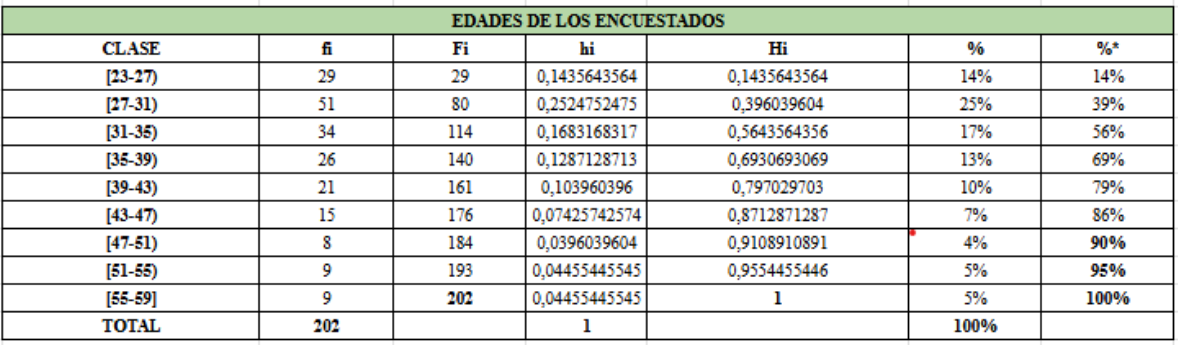
\includegraphics[width=0.80\textwidth]{images/edadencuestados.png}
            \end{center}
            \label{fig:edadencuestados}
        \end{figure}
        \begin{figure}[H]
            \begin{center}
                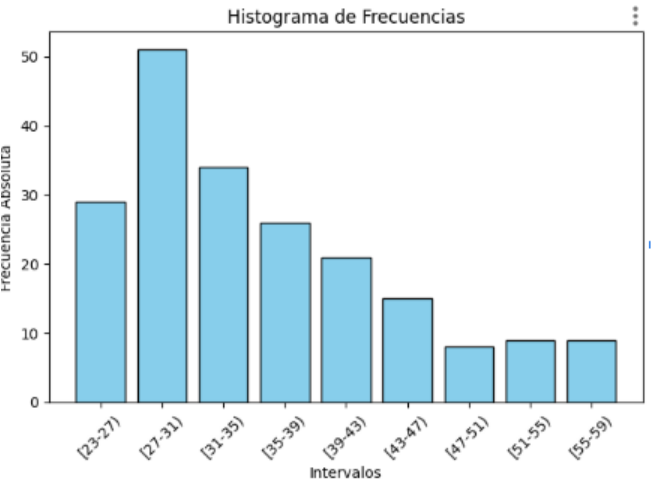
\includegraphics[width=0.80\textwidth]{images/histogramaEdad.png}
            \end{center}
            \label{fig:histogramaEdad}
        \end{figure}
        \begin{figure}[H]
            \begin{center}
                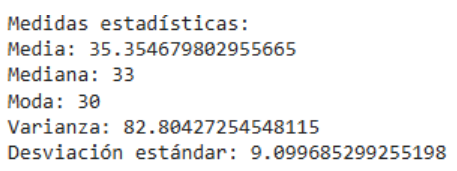
\includegraphics[width=0.80\textwidth]{images/EstadEdad.png}
            \end{center}
            \label{fig:EstadEdad}
        \end{figure}
        \item SEXO DE LOS ENCUESTADOS
        \begin{figure}[H]
            \begin{center}
                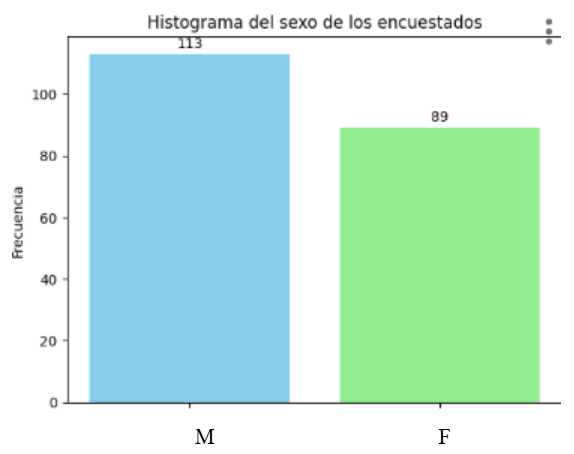
\includegraphics[width=0.80\textwidth]{images/frecuenciaGenero.png}
            \end{center}
            \label{fig:frecuenciaGenero}
        \end{figure}
        \begin{figure}[H]
            \begin{center}
                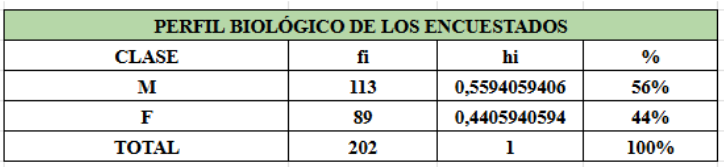
\includegraphics[width=0.80\textwidth]{images/PerfilBiologico.png}
            \end{center}
            \label{fig:PerfilBiologico}
        \end{figure}
        \item ESTADO CIVIL DE LOS ENCUESTADOS
        \begin{figure}[H]
            \begin{center}
                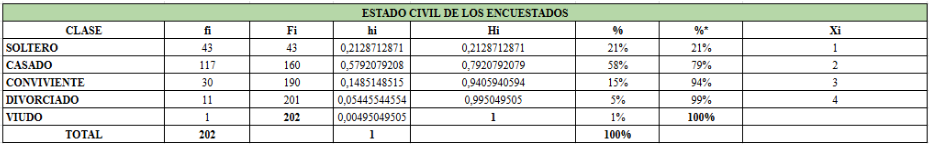
\includegraphics[width=0.80\textwidth]{images/EstadoCivil.png}
            \end{center}
            \label{fig:EstadoCivil}
        \end{figure}
        \begin{figure}[H]
            \begin{center}
                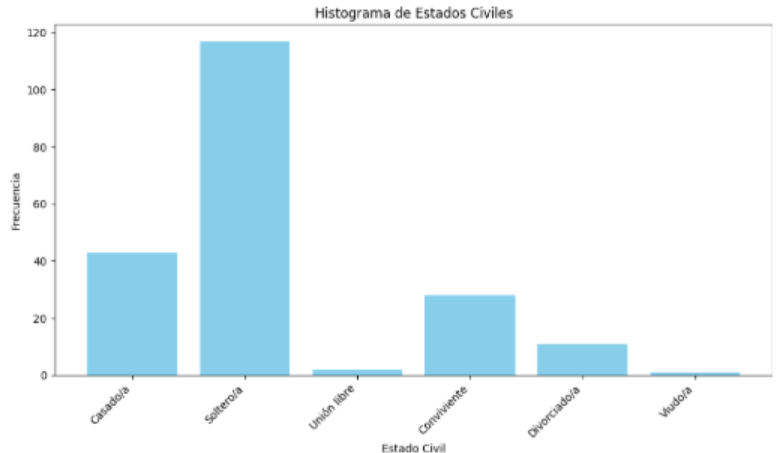
\includegraphics[width=0.80\textwidth]{images/histogramaEstadoCivil.png}
            \end{center}
            \label{fig:histogramaEstadoCivil}
        \end{figure}
        \begin{figure}[H]
            \begin{center}
                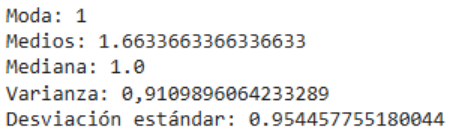
\includegraphics[width=0.80\textwidth]{images/EstadisticosEC.png}
            \end{center}
            \label{fig:EstadisticosEC}
        \end{figure}
        \item NIVELES DE ESTUDIO DE LOS ENCUESTADOS
        \begin{figure}[H]
            \begin{center}
                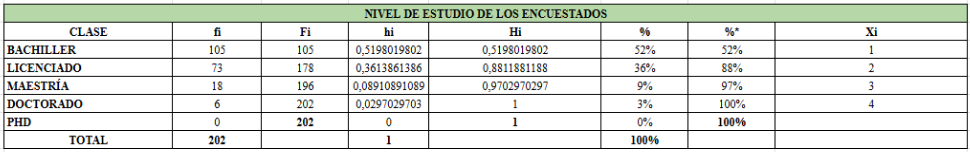
\includegraphics[width=0.80\textwidth]{images/nivelestios.png}
            \end{center}
            \label{fig:nivelestios}
        \end{figure}
        \begin{figure}[H]
            \begin{center}
                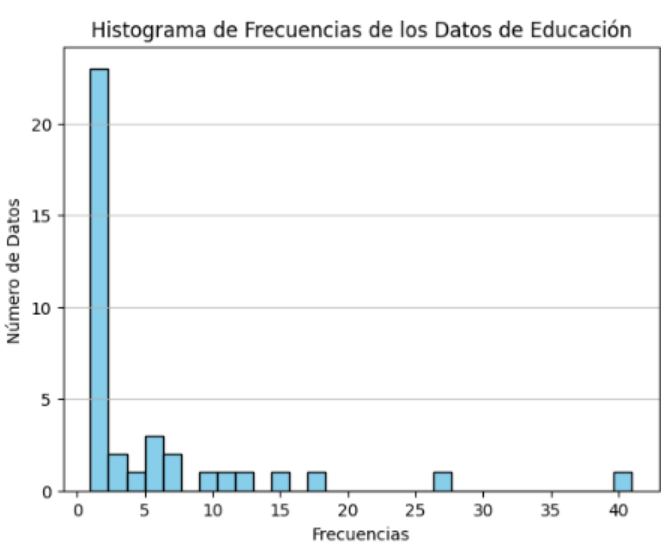
\includegraphics[width=0.80\textwidth]{images/NIvelHistograma.png}
            \end{center}
            \label{fig:NIvelHistograma}
        \end{figure}
    \end{enumerate}
    \item \textbf{SITUACIÓN DE EMPLEO}
    \begin{enumerate}
        \item SE ENCUENTRA EMPLEADO
        \begin{figure}[H]
            \begin{center}
                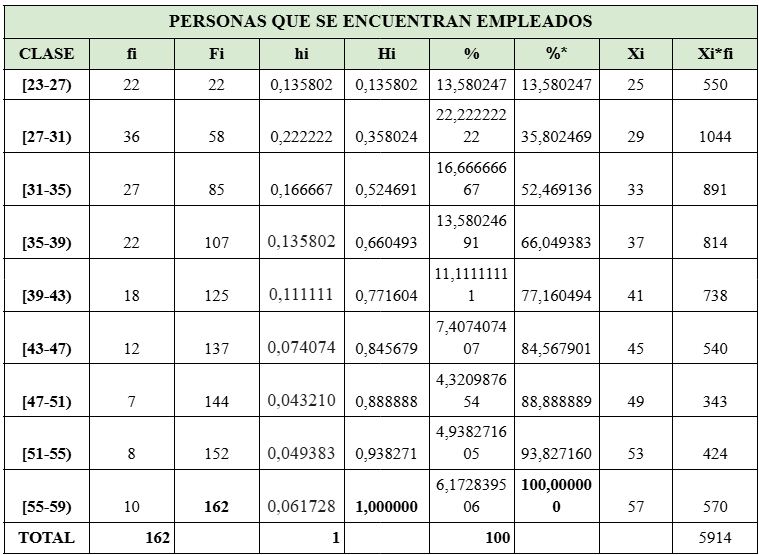
\includegraphics[width=0.80\textwidth]{images/frecuenciaempleados.png}
            \end{center}
            \label{fig:frecuenciaempleados}
            \caption{PERSONAS QUE SE ENCUENTRAN EMPLEADOS}
        \end{figure}
        \begin{figure}[H]
            \begin{center}
                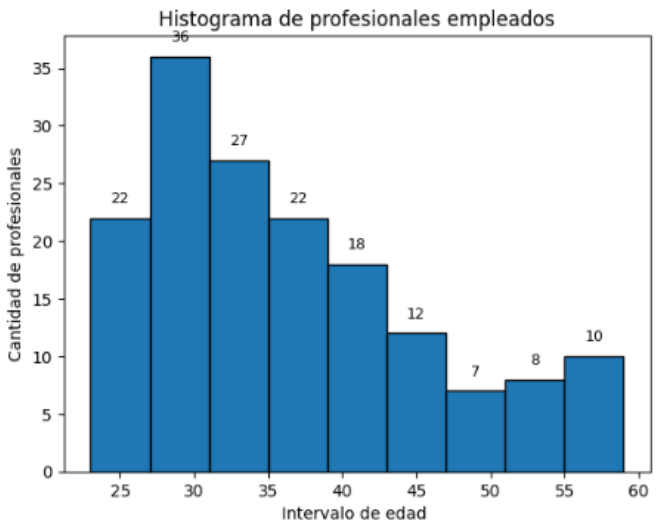
\includegraphics[width=0.80\textwidth]{images/HistogramEmpleados.png}
            \end{center}
            \label{fig:HistogramEmpleados}
        \end{figure}
        La moda es aproximadamente 29.43 años, lo que significa que el intervalo de edad con mayor concentración de profesionales es [27, 31). Este intervalo tiene la mayor frecuencia (36 profesionales), lo que indica que la mayoría de los empleados tienen entre 27 y 30 años.

        La varianza es de 86.27 años, lo que indica que hay una dispersión moderada de las edades en torno a la media. Este valor refleja cuánto varían las edades de los empleados respecto al valor promedio de 36.51 años.

        La desviación estándar es 9.29 años, lo que nos dice que, en promedio, las edades de los profesionales empleados se desvían en unos 9 años respecto a la media de 36.51 años.
        \item PROFESIONES ESTUDIADAS DE LOS PROFESIONALES EMPLEADOS
        \begin{figure}[H]
            \begin{center}
                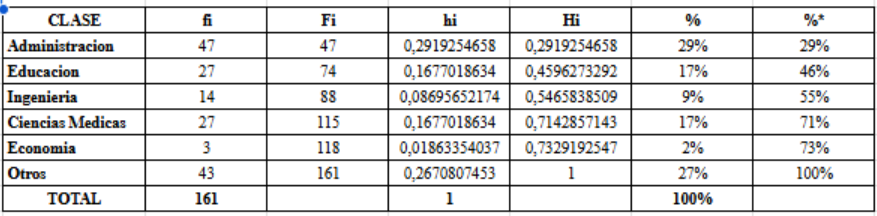
\includegraphics[width=0.80\textwidth]{images/profesionesEst.png}
            \end{center}
            \label{fig:profesionesEst}
        \end{figure}
        \begin{figure}[H]
            \begin{center}
                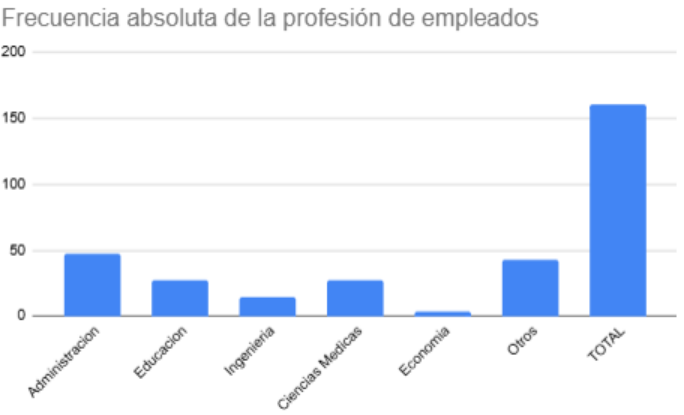
\includegraphics[width=0.80\textwidth]{images/frecuenciaemple21.png}
            \end{center}
            \label{fig:frecuenciaemple21}
        \end{figure}
INTERPRETACIÓN:
        En el distrito de Huánuco, se analizaron las profesiones de las personas empleadas, obteniéndose los siguientes resultados.

MODA:
La moda es Administración ya que estas profesiones tienen la mayor frecuencia absoluta (fi= 47), representando el 29\% del total de empleados.
Esto indica que la mayoría de las personas con empleo en el distrito estudiaron carreras relacionadas con administración, lo que sugiere que este sector es el más empleado

MEDIANA:
La mediana  corresponde a Ingenieria. Esto se debe a que el valor central de las frecuencias acumuladas (n/2=80.5) se encuentra dentro de esta categoría (Fi=88). 
Esto implica que, al ordenar las profesiones de los empleados del distrito, la profesión central pertenece al area de Ingenieria

        \item PROFESIONALES QUE EJERCEN SU PROFESIÓN
        \begin{figure}[H]
            \begin{center}
                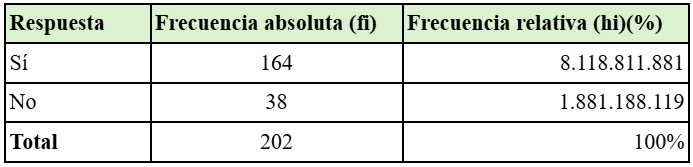
\includegraphics[width=0.80\textwidth]{images/empleo2.png}
            \end{center}
            \label{fig:empleo2}
        \end{figure}
        \begin{figure}[H]
            \begin{center}
                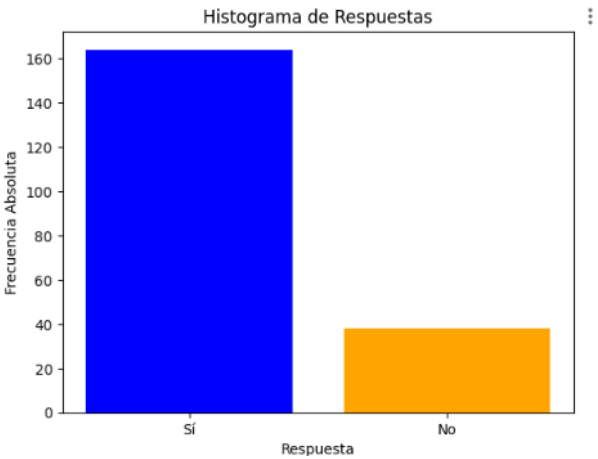
\includegraphics[width=0.80\textwidth]{images/ejercenHist.png}
            \end{center}
            \label{fig:ejercenHist}
        \end{figure}

        Media: La media indica que en promedio el 81.2 de las respuestas son Sí.
Moda: La confirma que la respuesta más frecuente es “Sí “, nos da entender que mas de 80\% de los encuestados ejercen su profesión.
 Mediana: La mediana es Sí por que posiciones 101 y 102 en el conjunto de datos corresponde a la respuesta Sí. La media es un valor que divide el conjunto de datos en dos partes, en este caso la mitad de los datos se encuentras dentro de la respuesta Sí.
Varianza: La varianza es 7938.5 lo que indica que las respuestas están dispersas, en este caso la varianza es bastante alta lo que indica que existe una diferencia considerable entre las frecuencias de las respuestas Si y No.
 Desviación estándar: La desviación estándar de 89.10 es demasiado alta, lo que indica que una considerable dispersión en las respuestas. Es decir que hay una diferencia significativa entre las frecuencias de Sí y No. aunque la mayoría de las respuestas es Si, desviación estándar refleja la variabilidad de las respuestas en relación con la media.
        \item SECTOR DE TRABAJO DE LOS PROFESIONALES
        \begin{figure}[H]
            \begin{center}
                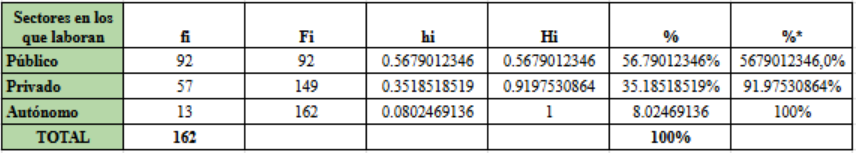
\includegraphics[width=0.80\textwidth]{images/trabajoprofesiones.png}
            \end{center}
            \label{fig:trabajoprofesiones}
        \end{figure}
        \begin{figure}[H]
            \begin{center}
                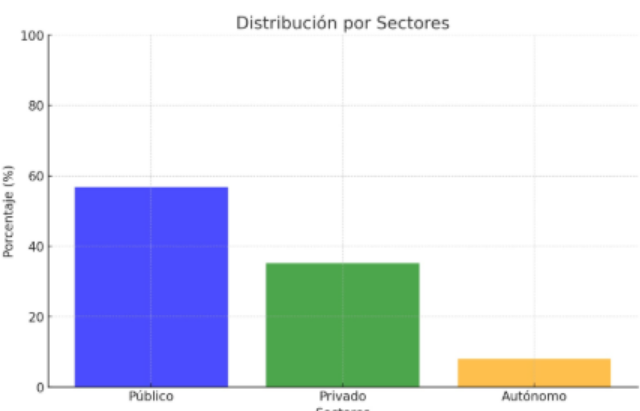
\includegraphics[width=0.80\textwidth]{images/distribucionSectores.png}
            \end{center}
            \label{fig:distribucionSectores}
        \end{figure}
        Media:
La media de los porcentajes de los sectores laborales es 33.33\%. Esto significa que, en promedio, la participación de cada sector en el total de personas laborando es del 33.33\%. Sin embargo, este promedio no refleja la distribución real, ya que el sector público tiene una representación significativamente mayor.

Mediana:
La mediana también corresponde al sector público. Esto se debe a que el valor central de las frecuencias acumuladas (n/2=81) se encuentra dentro de este sector (fi=92). Esto implica que, al ordenar los sectores laborales, el sector público se ubica en la posición central, reflejando su predominancia en la distribución.

    \end{enumerate}
    \item INTERPRETACIÓN
    Sector Público: Más de la mitad de los encuestados en la región de Huánuco (56.79\%) trabaja en el sector público, consolidándose como el principal generador de empleo en la zona.
    Sector Privado: El 35.18\% de los encuestados labora en el sector privado, destacándose como una importante fuente de empleo en la región.
    Sector Autónomo: Solo el 8.02\% de los encuestados se dedica a actividades independientes, reflejando una menor participación en este ámbito laboral.

    \item EJERCE SU PROFESIÓN
    \begin{figure}[H]
        \begin{center}
            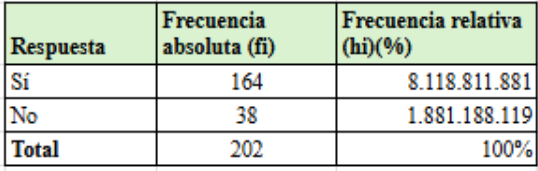
\includegraphics[width=0.80\textwidth]{images/ejerceProfesion.png}
        \end{center}
        \label{fig:ejerceProfesion}
    \end{figure}
    \item SITUACIÓN DE DESEMPLEO
    NO SE ENCUENTRA EMPLEADO
    \begin{figure}[H]
        \begin{center}
            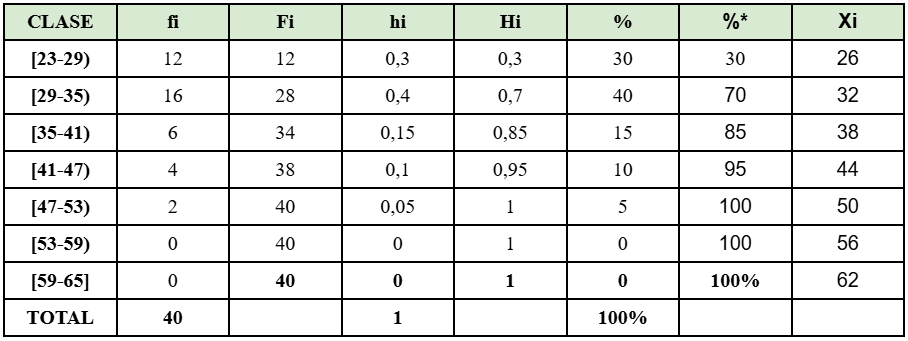
\includegraphics[width=0.80\textwidth]{images/noEncuentra.png}
        \end{center}
        \label{fig:noEncuentra}
    \end{figure}
    \begin{figure}[H]
        \begin{center}
            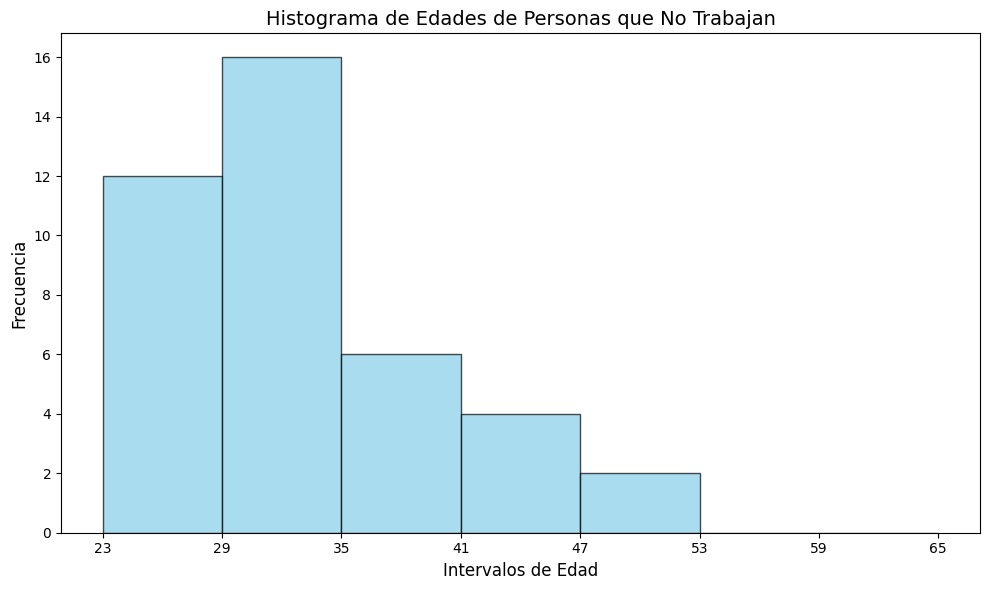
\includegraphics[width=0.80\textwidth]{images/johan.jpg}
        \end{center}
        \label{fig:noEcHist}
    \end{figure}

    Interpretación de los datos obtenidos:

Tabla de Frecuencias:
fi 2 : 16 personas del total de desempleados tienen entre 29 - 34 años, entonces podemos deducir que la mayoría de las personas que tienen entre esas edades se encuentran desempleados.
fi 5 : 2 personas del total de desempleados tienen entre 47 - 53 años, entonces podemos deducir que las personas que tienen entre esas edades tienen más posibilidades de tener empleo.

Medidas Obtenidas:

MEDIA: 33.2 es el promedio de las personas que se encuentran desempleadas 
MEDIANA: De las 40 personas desempleadas, la mitad tiene menos de 32 años y la otra mitad tiene más de 32 años.
MODA: Significa que la edad más frecuente del total de personas desempleadas que se está analizando es de aproximadamente 26 años.  
VARIANZA: Significa que la edad más frecuente del total de personas desempleadas que se está analizando es de aproximadamente 31 años.  
    \item PROFESIONES ESTUDIADAS DE LOS PROFESIONALES DESEMPLEADOS
    \begin{figure}[H]
        \begin{center}
            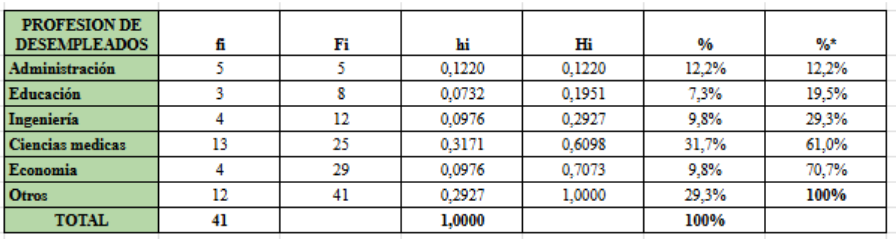
\includegraphics[width=0.80\textwidth]{images/fram.png}
        \end{center}
        \label{fig:fram}
    \end{figure}
    \begin{figure}[H]
        \begin{center}
            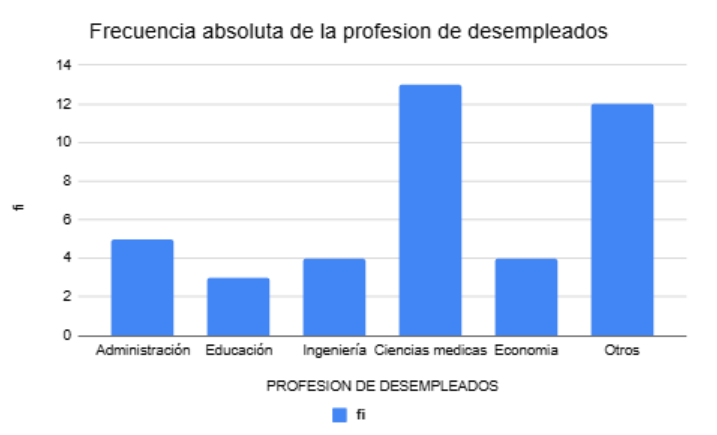
\includegraphics[width=0.80\textwidth]{images/fram2.png}
        \end{center}
        \label{fig:fram2}
    \end{figure}
    MODA: La moda es la categoría con mayor frecuencia absoluta (fi). De la tabla, la categoría con mayor fi es Ciencias Médicas, con fi =13. Moda: Ciencias Médicas.
MEDIANA: La mediana se encuentra en la categoría donde está el valor central de las frecuencias acumuladas (Fi). El total de frecuencias es 41, y el valor central es n / 2 = 41 / 2 = 20.5. Buscamos en la columna Fi: Fi = 25 para Ciencias Médicas incluye el valor 20.5. Por lo tanto, la mediana es: Mediana: Ciencias Médicas	.
Interpretación de los resultados: En el distrito de Huánuco, se analizaron las profesiones de las personas desempleadas, obteniéndose los siguientes resultados:
Mediana:
La mediana también corresponde a Ciencias Médicas. Esto se debe a que el valor central de las frecuencias acumuladas (n/2=20.5) se encuentra dentro de esta categoría (Fi=25).  Esto implica que, al ordenar las profesiones de los desempleados del distrito, la profesión central pertenece también al área de la salud.	
Moda:
La moda es Ciencias Médicas, ya que esta profesión tiene la mayor frecuencia absoluta (fi= 13), representando el 31.7\% del total de desempleados.
Esto indica que la mayoría de las personas sin empleo en el distrito estudiaron carreras relacionadas con el área de salud, lo que sugiere que este sector es el más afectado por el desempleo.
\item PRINCIPALES OBSTÁCULOS PARA CONSEGUIR EMPLEO
\begin{figure}[H]
    \begin{center}
        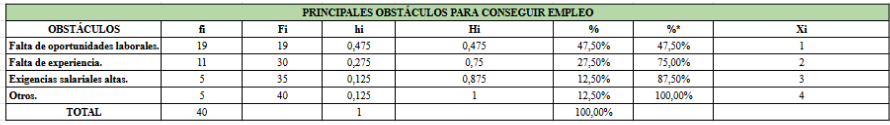
\includegraphics[width=0.80\textwidth]{images/obst.png}
    \end{center}
    \label{fig:obst}
\end{figure}
\begin{figure}[H]
    \begin{center}
        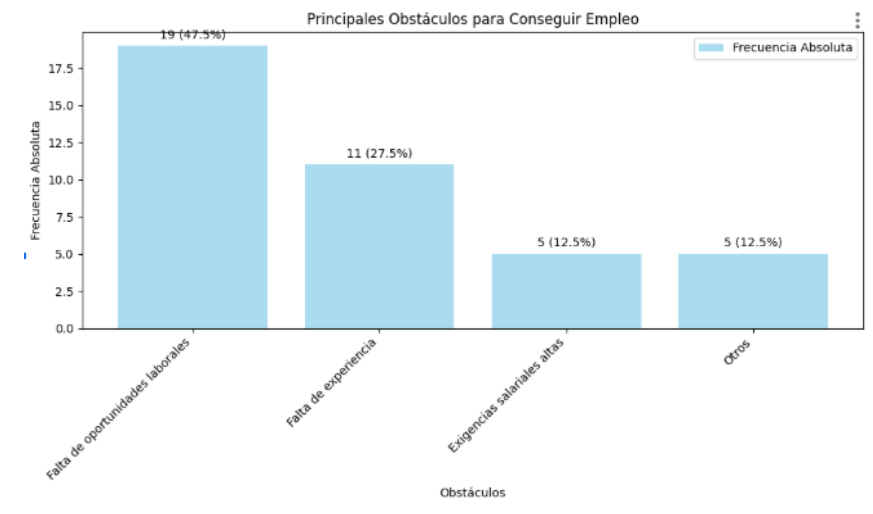
\includegraphics[width=0.80\textwidth]{images/obs21.png}
    \end{center}
    \label{fig:obs21}
\end{figure}
ANÁLISIS:
La media hallada sugiere que el promedio de los obstáculos para encontrar empleo se encuentra expresado en el valor de 1, que indica el obstáculo “falta de oportunidades laborales” y aporta el hecho de que los datos recopilados muestran una tendencia de preferencia, en un segundo lugar al obstáculo “falta de experiencia”. Lo que nos sugiere la marcada preferencia por los obstáculos de mínimos valores, que son los dos primeros de la lista. Lo que nos indica sobre la percepción de los encuestados sobre la dificultad para encontrar empleo, que es mayoritaria la asignación de la dificultad para obtener empleo en la realidad externa (fenómenos y hechos sociales, económicos y políticos), que en la interna (razones individuales).

El valor de la media de 20.5 nos indica que el dato que tiene el orden 20.5° se encuentra en el intervalo de la frecuencia acumulada que contiene el 20.5\% de datos. El dato 20,5° se encuentra en el intervalo de “Falta de Oportunidades Laborales” al contar con una frecuencia de 19 en tal intervalo y empezar en 30 frecuencias en el siguiente. Esta cifra, nuevamente nos ubica en la preferencia de “falta de oportunidades laborales” por la mayoría de encuestados como dificultad de empleo.

El valor de la media de 20.5 nos indica que el dato que tiene el orden 20.5° se encuentra en el intervalo de la frecuencia acumulada que contiene el 20.5\% de datos. El dato 20,5° se encuentra en el intervalo de “Falta de Oportunidades Laborales” al contar con una frecuencia de 19 en tal intervalo y empezar en 30 frecuencias en el siguiente. Esta cifra, nuevamente nos ubica en la preferencia de “falta de oportunidades laborales” por la mayoría de encuestados como dificultad de empleo.


\end{enumerate}


\section{CONCLUSIONES}
Se logró el objetivo general de conocer la situación de empleo y desempleo de los profesionales del distrito de Huánuco en el año 2024. Se lograron los objetivos específicos de la investigación: conocer la cantidad de profesionales empleados y desempleados del distrito de Huánuco en el 2024 según sus edades; conocer las profesiones estudiadas por los profesionales empleados; conocer cuántos profesionales empleados del distrito de Huánuco en el año 2024 ejercen su profesión; conocer el área de trabajo de los profesionales del distrito de Huánuco en el 2024; conocer la perspectiva de los profesionales del distrito de Huánuco consultados cuáles son los obstáculos principales para encontrar empleo; conocer las profesiones estudiadas por los profesionales desempleados del distrito de Huánuco en el año 2024. Se concluye que la cantidad de profesionales empleados en el distrito de Huánuco es mayor a la de los profesionales desempleados, que existe una tasa mayor de profesionales empleados que trabajan en el sector público, que las carreras profesionales con mayor cantidad empleados es la de ciencias administrativas, seguida de educación y ciencias de la salud. Al mismo tiempo, las carreras relacionadas a las ciencias de la salud muestran una mayor cantidad de desempleados. Y que, el principal obstáculo de  obtención de empleo es la falta de oportunidades laborales, considerado por los profesionales del distrito de Huánuco, en el año 2024, lo que parece indicar una escasez de empleo en nuestra localidad.


\section{REFERENCIAS BIBLIOGRÁFICAS}

Rengifo Pizango, L. A., y Yume Lancha, R. D. (2024). Percepción de empleabilidad en estudiantes de un curso de titulación en una universidad privada de Lima. Tesis de licenciatura, Universidad Marcelino Champagnat, Lima, Perú. Recuperado de https://repositorio.umch.edu.pe/handle/20.500.14231/3725

Muñoz Izquierdo, C. (2020). Determinantes de la empleabilidad de los jóvenes universitarios y alternativas para promoverla. Revista de Psicología Política, 12(49), 1-10. Recuperado de https://www.scielo.org.mx

Rosas Ruiz, G. M. (2023). Título de la investigación. Tesis de licenciatura, Universidad de Huánuco, Perú. Recuperado de https://repositorio.udh.edu.pe/bitstream/handle/20.500.14257/4184/Rosas\%20Ruiz\%2c\%20Gianella\%20Mal\%c3\%ba.pdf?sequence=1\&isAllowed=y

Keynes, J. M. (1936). Teoría general de la ocupación, el interés y el dinero. En este texto, Keynes critica la teoría clásica y argumenta que el nivel de empleo está determinado por la demanda agregada en la economía.

\end{document}